\section{Introduction}
\begin{itemize}
    \item Last section was about OSI layer 2, IP addresses, subnetmasks, etc.
    \item In this section we are still in layer 3 and we are going to go much deeper, and learn to control the boundaries.
\end{itemize}


%----------------------------------------------------------------------------------------
\section{CIDR - Classless Inter-Domain Routing}
\begin{itemize}
    \item CIDR - Classless Inter-domain routing:
        \begin{itemize}
            \item A problem with classful addresses was that if a company had more than 254 hosts they would need to be assigned a class B network.
                \begin{itemize}
                    \item The internet authorities gave class A,B,C,D,E addresses. If they had 500 hosts they would get addresses for 65,543 hosts because the next class would allocate the whole next octet of the host portion. This was a waste.
                \end{itemize}
            \item They would have much less than the 65,434 hosts allocated, so this wasted a huge amount of the global address space.
            \item Classless inter-domain routing (CIDR) was introduced in 1993 to alleviate this problem.
                \begin{itemize}
                    \item This removed the problem of classful addresses only allocating octets and instead allowed them to be split into smaller networks.
                \end{itemize}
            
            \item CIDR removed the fixed /8, /16, and /24 requirements for the address classes, and removed them to be split or 'subnetted' into smaller networks. For example 172.10.10.0 /20.
            \item Companies can now be allocated an address range which more closely matches their needs and does not waste addresses.
            \item The name for this is \textbf{subnetting}.
            \item The benefit of Subnetting is that we don't waste addresses.
        \end{itemize}
    
    \item CIDR and Route summarisation:
        \begin{itemize}
            \item Another benefit of CIDR is that aggregate blocks of networks can be advertised on the internet.
            \item For example lets say that a company called 'ISP A' gets assigned from the internet authorities the range of IP addresses ranging from 175.10.0.0/24 - 175.10.255.0. We also have another company called 'ISP B' are given 175.11.0.0/24 - 175.11.255.0/24.
            \item Now these companies connect to each other and when CIDR comes in that ISP A and ISP B would need to copy all the routes from its routers and advertise all their 256 address blocks to each other, but when we have CIDR we just summarize the bits that they have in common so that we dont have duplicate data in the routing tables. 
            \item In this case ISP A would advertise 175.10.0.0/16 to ISP B, and now ISP B only learns one router to get to ISP A rather than learning 256 routes. This is complicated and vaguely explained in this lecture, so watch the youtube video below.
            \item This was actually not very well explained in the course so this youtube video actually cleared it up: \url{https://www.youtube.com/watch?v=YOpwKwol8xk}
        \end{itemize}
    
    \item Route summarization benefits:
        \begin{itemize}
            \item ISP A does not know about all 256 /24 networks reachable in ISP B. 
            \item It only has the single 175.11.0.0/16 summary route. It has 1 route instead of 256. Less memory is used.
            \item This reduces the size of ISP A's routing table and takes up less memory.
            \item If an individual link goes down in ISP B, it has no impact on ISP A. The single summary route does not change.
            \item (Routers in ISP B would have to recalculate their routing table if a link went down)
            \item This restricts issues to the local part of the network and reduces CPU overload.
        \end{itemize}
\end{itemize}


%----------------------------------------------------------------------------------------
\section{Subnetting overview}
\begin{itemize}
    \item Subnetting:
        \begin{itemize}
            \item Subnetting is one of the core knowledge areas in networking, crucial for the CCNA and for networking in general.
            \item To understand this lecture, think about it from the point of view of the originally intended IP4 design again, where all hosts which can communicate on the internet have a public IP address.
                \begin{itemize}
                    \item Think of it 10-15 years ago when people did not have problems with IP address shortage.
                \end{itemize}
            \item Let's say we're the network designer fro a small business with four departments spread over two offices, and we want to manage our own public address space.
                \begin{itemize}
                    \item We could buy 4 separate class C networks for that. But the problem is that public IP addresses are expensive.
                \end{itemize}
            \item Rather than purchasing separate address ranges for the different departments, we can purchase a single class C range and subnet it into smaller portions. And then we can subnet that to the different departments of our network.
        \end{itemize}
    
    \item Borrowing host bits:
        \begin{itemize}
            \item Let's say we've been allocated class C 200.15.10.0/24.
                \begin{figure}[H]
                    \centering
                    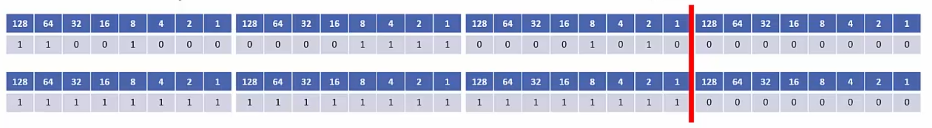
\includegraphics[width=0.4\textwidth]{./figs/2022-01-16-21-17-47.png}
                % 	\caption{}
                \end{figure}
            
            \item To subnet the network into smaller subnets, we need to 'borrow' host bits and add them to the network portion of the address. 
                \begin{itemize}
                    \item We are going to move the border of the subnetmask to the right. 
                    \item WHEN WE ARE DOING SUBNETTING THE LINE ALWAYS MOVES TO THE RIGHT.
                \end{itemize}
            \item The network address line always moves to the right when we subnet. 
            \item The further to the right we go, the more subnets we'ññ have of that size but less hosts.
        \end{itemize}
    
    \item To calculate the number of networks:
        \begin{itemize}
            \item To calculate the number of available subnets, the formula is $\displaystyle 2^{\text{subnet-bits}}$.
            \item If a class C network uses a 28 subnet mask then we've borrowed 4 bits from the default of /24.
            \item $\displaystyle 2^4 = 16$ available subnets.
            \item If a class B network uses a /28 subnet mask then we've borrowed 12 bits from the default of /16.
            \item $\displaystyle 2^{12} = 4096$ available subnets.
            \item Hosts on different subnets need to go via a router if they want to communicate with each other.
        \end{itemize}
    
    \item To calculate the number of hosts:
        \begin{itemize}
            \item To calculate the nuber of available hosts, the formula is $\displaystyle 2^{\text{ host-bits }} - 2$.
            \item We subtract 2 because the network address and broadcast address cannot be assigned to hosts.
            \item If a class C network uses a /28 subnet mask then we have 4 bits left for hosts.
            \item $\displaystyle 2^4-2=14$ 
            \item If a class B network uses a /28 subnet mask then we have 4 bits left for hosts.
            \item The amount of hosts we get is going to be dependant on the subnet size.
        \end{itemize}
    
    \item A quick note on \verb|ip subnet-zero| command:
        \begin{itemize}
            \item Just like we have to subtract 2 to get the number of valid hosts, we used to have to subtract 2 to get the number of available networks also. 
            \item In the original internet standards, it was not allowed to use network bits of all 0's or all 1's (just like we can't use all host bits of all 0's or all 1's).
            \item There wasn't really any practical need for this and it wasted address space.
            \item The \verb|ip subnet-zero| command on a router overrides the limitation, and is enabled by default.
            \item This is important because on the updated standards we don't use the 2 subnets we use to take off for the network, we ONLY DO THIS FOR THE HOSTS. Hence, you DO NOT SUBTRACT 4, you subtract 2. Do not do that for the CCNA.
        \end{itemize}
\end{itemize}


%----------------------------------------------------------------------------------------
\section{Subnetting classs C networks and VLSM}
\begin{itemize}
    \item Class C /31 subnet:
        \begin{itemize}
            \item Let's say we've been allocated class C 200.15.10.0/24.
            \begin{figure}[H]
                \centering
                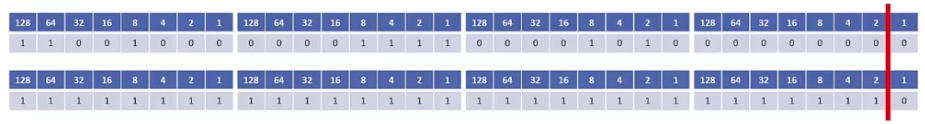
\includegraphics[width=0.4\textwidth]{./figs/2022-02-14-13-14-18.png}
            % 	\caption{}
            \end{figure}
            \begin{itemize}
                \item If we want to have any hosts available then the highest subnetmask we can have is /31. In that case we leave 1 bit remaining for the hosts.
            \end{itemize}
        \item If we move the line all the way to the right we're now using /31 (or 255.255.255.254).
        \item This leaves one bit for the host address, with a possible value of 0 or 1.
        \item It borrows 7 bits from the network address.
        \item This gives us 128 subnets $\displaystyle 2^7$ which accommodates 2 hosts each.
        \item We subnet using /31. Valid host addresse:
            \begin{itemize}
                \item 200.15.10.0 to 200.15.10.1
                \item 200.15.10.2 to 200.15.10.3
                \item etc. to: 
                \item 200.15.10.254 to 200.15.10.255
            \end{itemize}
        
        \item Notice that the first three octets never change. The subnet mask changes in the first 7 bits.
        \item What about the network and broadcast address?
            \begin{itemize}
                \item /31 breaks the standard rules of IP addressing.
                \item /31 subnets are supported in cisco routers for point to point links (which have no need for a network or broadcast address).
                    \begin{itemize}
                        \item A point to point link means that all traffic moves from one to the other in terms of all messages sent can only be sent to the one other host in that subnet. There is no other place for the message to go so this is why we don't need a broadcast and network address. 
                        \item This is why cisco allowed that exception, we can have a /31 subnet mask on a point to point link.
                    \end{itemize}
            \end{itemize}
        \end{itemize}

    \item Class C /31 subnet mask:
        \begin{itemize}
            \item Let's say we've been allocated a class C 200.15.10.0/24.
            \item Let's move the line back a place. We're now using /30 (or 255.255.255.252).
            \item This leaves 2 bits for the host address, $\displaystyle 2^2-2=2$ hosts available and the network and broadcast address.
            \item It borrows 6 bits for the network address.
            \item This gives us 64 subnets $\displaystyle 2^6$ which accommodate 2 hosts each.
            \item Notice that the line is after the 4. The network addres goes up in values of 4.
                \begin{figure}[H]
                    \centering
                    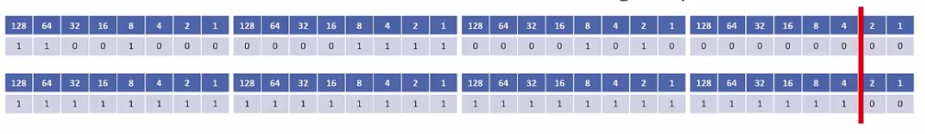
\includegraphics[width=0.4\textwidth]{./figs/2022-02-14-13-28-13.png}
                % 	\caption{}
                \end{figure}
            
            \item Valid hosts addresses:
                \begin{itemize}
                    \item 200.15.10.1 to 200.15.10.2 (network .0, broadcast .3).
                    \item 200.15.10.5 to 200.15.10.6 (network .4, broadcast .7).
                    \item etc. to:
                    \item 200.15.10.253 to 200.15.10.254 (network .252, broadcast .255).
                \end{itemize}
            
            \item 
        \end{itemize}
\end{itemize}

\subsection{/31 vs /30}
\begin{itemize}
    \item /31 and /30 both accommodate 2 hosts per subnet. Because /31 subnets dont have a network and broadcast address.
    \item /31 supports 128 subnets, /30 only 64.
    \item /31 us useful if you need to maximize use of your address space.
    \item /30 is more standard and commonly used.
    \item For the CCNA exam, use /30 when a subnet to support 2 hosts is required, unless told to use /31. 
        \begin{itemize}
            \item Because usually a /30 is the correct answer. Only to maximize use /31, otherwise always use /30.
        \end{itemize}
\end{itemize}

\subsection{Class C /29 subnet}
\begin{itemize}
    \item Let's say we've been allocated Class C 200.15.10.0/24.
        \begin{figure}[H]
            \centering
            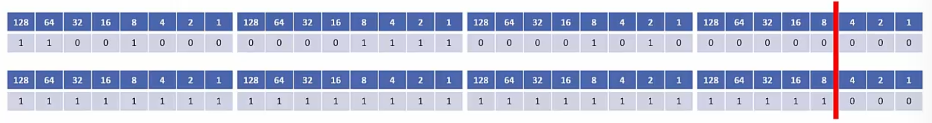
\includegraphics[width=\width\textwidth]{./figs/20220610123227.png}
        \end{figure}
    \item Let's move the line back a place. We've now using /29 (or 255.255.255.248).
    \item This leaves 3 bits for the host addresses, $\displaystyle 2^3 - 2 = 6$ possible hosts.
    \item It borrows 5 bits for the network address.
    \item This gives us 32 subnets $\displaystyle 2^5$ which accommodate 6 hosts each.
    \item The valid host addresses are:
        \begin{itemize}
            \item 200.15.10.1 to 200.15.10.6 (network .0, broadcast .7)
            \item 200.15.10.9 to 200.15.10.14 (network .8, broadcast .15)
            \item etc. to:
            \item 200.15.10.249 to 200.15.10.254 (network .248, broadcast .255)
        \end{itemize}
\end{itemize}

\subsection{Other class C subnet masks}
\begin{itemize}
    \item We can carry on moving the red line back a place.
    \item We can do for example: 
        \begin{itemize}
            \item /28 or (255.255.255.240) = 16 networks of 14 hosts each.
            \item /27 or (255.255.255.224) = 8 networks of 30 hosts each.
            \item /26 or (255.255.255.192) = 4 networks of 62 hosts each.
            \item /25 or (255.255.255.128) = 2 networks of 126 hosts each.
            \item /24 or (255.255.255.0) = 1 network of 254 hosts (the default, no subnetting).
        \end{itemize}
\end{itemize}


%----------------------------------------------------------------------------------------
\section{Subnetting practice questions}
\begin{itemize}
    \item What are the network address, broadcast address, and valid host address for the IP address 198.22.45.173/26?
        \begin{itemize}
            \item 198.22.45.173 = \hl{11000110.00010110.00101101.10}101101
            \item The highlighted part is the /26, we cannot do anything with those bits, only with the reamining.
            \item The network and broadcast addresses:
                \begin{tabular}{|c|c|}
                    \hline
                    Network address & Broadcast address \\
                    \hline
                        \hl{11000110.00010110.00101101.10}000000 & 
                        \hl{11000110.00010110.00101101.10}111111 \\
                    \hline
                        198.22.45.128 &
                        198.22.45.191
                     \\
                    \hline
                \end{tabular}
            
            \item The valid host addresses: 198.22.45.129 - 198.22.45.190.
        \end{itemize}

    \item What is the subnet mask in dotted decimal notation? 
        \begin{itemize}
            \item 255.255.255.192
        \end{itemize}
    
    \item Note that when we subnet a class C address the magic is all going to happen in the last subnet.
    \item So we didn't really need to write out the 198.22.45 part.
\end{itemize}

%%%%%%%%%%%%%%%%%%%%%%%%%%%%%%%%%%%%%%%%%%%%%%%%%%%%%%
\section{Variable Length Subnet Masksking Example 1}
\begin{itemize}
    \item Early routing protocols only supported fixed length subnet masking (FLSM) where all the subnets had to be the same size. You couldn't have a subnet with 14 hosts and another with 64 hosts in the same network.
        \begin{itemize}
            \item If you had a subnet that was /28 they all had to be /28 no /27 or any other submask within the same larger network.
            \item Now variable length subnet masks are supported.
        \end{itemize}
        
    \item All modern routing protocols support variable length subnet masking. This allows us to size subnets differently according to how many hosts they have. 
\end{itemize}

\subsection{Subnetting considerations}
\begin{itemize}
    \item How many locations do we have in the network?
    \item How many hosts are in each location?
    \item What are the IP addressing requirements fro each location? (Should different department types of host be in different subnets?)
    \item What size is appropriate for each subnet? (Don't waste addresses, but leave room for growth)
        \begin{itemize}
            \item Don't make it too big, and don't make it too slow as to have to make a topology redesign later.
        \end{itemize}
\end{itemize}

\subsection{Network topology diagram}
\begin{itemize}
    \item We have a network topology diagram, we have an organization with an office in NY, another one in Boston, NY is the headquarters, they have 14 hosts in the sales department and 28 hosts in the engineering department. In boston they have 28 in engineering and 7 in the sales department.
        \begin{figure}[H]
            \centering
            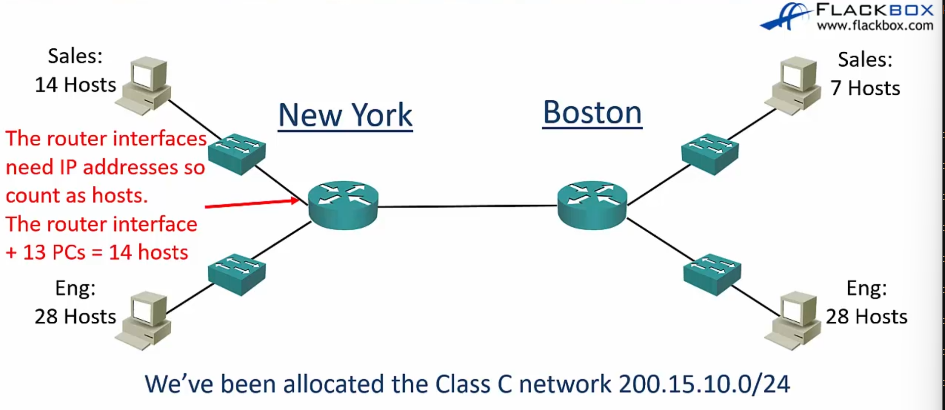
\includegraphics[width=\width\textwidth]{./figs/20220610143719.png}
        \end{figure}

    \item We've been allocated the class C network 200.15.10.0/24 from our internet service provider.
    \item We have Point to point link between the routers, this means that each of them are going to get one of the host ip addresses.
\end{itemize}

\subsection{Subnetting design steps}
\begin{itemize}
    \item Find the largest segments and allocate a suitable subnet size for it.
    \item Allocate this subnet at the start of the address space.
    \item Continue going down the list.
    \item In the real world you want a scalable design -- you will likely allocate spare subnets for future growth, and leave space in the subnets for additional hosts.
        \begin{itemize}
            \item Example: the engineering department we have 28 hosts, don't give the subnet that size because you never know if you might need mor in the future.
            \item Maybe you need 2 more hosts in the next month for new employees, you need to keep this in mind.
            \item And if you allocate 2 subnets of 30 for the engineering and sales, don't do this, instead leave 3 or 4 subnets of 30 hosts, because that way you have the capacity for growth and you don't need to redesign the topology later on, everything is still sequential and contigous and everything works.
            \item Don't design for what is required right now, leave some room for growth.
            \item THIS IS WHAT YOU DO IN THE REAL WORLD, IN THE EXAM DON'T THINK LIKE THIS. DO EXACTLY AS YOU ARE TOLD. Even if you think that would be a stupid thing to do.
        \end{itemize}
    \item In the CCNA exam do exactlu what the question asks, don't worry about wether it's best practice or not.
\end{itemize}

\subsection{Engineering departments}
\begin{itemize}
    \item The engineering deparments in both sites have 28 hosts.
    \item For our example we've been told that the departments will not grow and we need to use the smallest subnets possible to maximise our address space.
    \item Let's find the optimal subnetmask for the engineering departments, and determine the network and broadcast addresses of each.
\end{itemize}

\subsection{Engineering departments answer}
\begin{itemize}
    \item We've been allocated 200.15.10.0/24
        \begin{figure}[H]
            \centering
            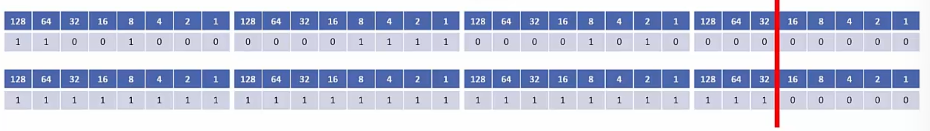
\includegraphics[width=\width\textwidth]{./figs/20220610144836.png}
            %\caption{}
        \end{figure}
    
    \item /27 or (255.255.255.224) supports 30 hosts. It is not 28 because we need the network address and the broadcast + the 28 hosts.
    \item New york engineering subnet:
        \begin{itemize}
            \item Network address: 200.15.10.0/27
            \item Broadcast address: 200.15.10.31
            \item Hosts 200.15.10.1-30.
        \end{itemize}
    
    \item Boston engineering subnet:
        \begin{itemize}
            \item Network address: 200.15.10.32/27
            \item Broadcast address: 200.15.10.63
            \item Hosts: 200.15.10.33-62
        \end{itemize}
\end{itemize}

%%%%%%%%%%%%%%%%%%%%%%%%%%%%%%%%%%%%%%%%%%%%%%%%%%%%%%
\section{Variable Length Subnet Masking Example Part 2}
\begin{itemize}
    \item We will go through the subnet for the rest of the departments.
\end{itemize}


\subsection{New York Sales Department}
\begin{itemize} 
    \item The question:
        \begin{itemize}
            \item The next largest subnet is New York Sales which requires 14 hosts.
            \item Pause the video here and calculate the optimal subnet mask.
            \item Also determine the network and broadcast addresses that we will allocate, and the range of host addreses.
        \end{itemize}
    
    \item We've allocated 200.15.10.0/24
        \begin{figure}[H]
            \centering
            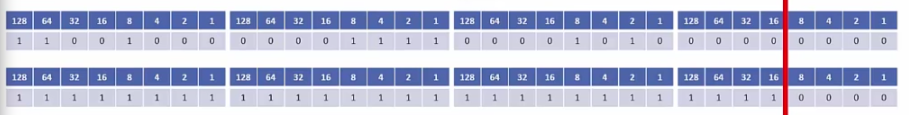
\includegraphics[width=\width\textwidth]{./figs/2022-10-19-22-53-45.png}
            %\caption{}
        \end{figure}
    
    \item /28 (0r 255.255.255.240) supports 14 hosts.
    \item 200.15.10.0 to 200.15.10.63 are already in use by the engineering departments, so this network address will start at 200.15.10.64.
    \item The network addresses goes up in values if 16, so the next one is 200.15.10.80.
    \item Our broadcast address is 200.15.10.79.
    \item Valid hosts addresses are 200.15.10.65 to 200.15.10.78.
\end{itemize}

\subsection{Boston Sales Department}
\begin{itemize}
    \item The question:
        \begin{itemize}
            \item The next largest subnet is Boston Sales which requires 7 hosts.
            \item Pause the video here and calculate the optimal subnet mask.
            \item Also determine the network and broadcast addresses that we will allocate, and the range of host addresses.
        \end{itemize}
    
    \item We've allocated 200.15.10.0/24
        \begin{figure}[H]
            \centering
            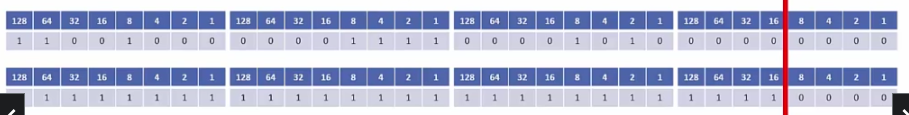
\includegraphics[width=\width\textwidth]{./figs/2022-10-19-23-13-11.png}
            %\caption{}
        \end{figure}
    \item /28 supports 14 hosts.
    \item /29 does not support 8 hosts because of the network and broadcast address.
    \item 200.15.10.0 to 299.15.10.79 are already in use, so this network address will start at 200.15.10.80.
    \item The network address goes up in valies of 16, so the next one is 200.15.10.96.
    \item Our broadcast address is 200.15.10.95.
    \item Valid host addresses are 00.15.10.81 to 200.15.10.94.
\end{itemize}

\subsection{Subnetting}
\begin{itemize}
    \item We are not done.
    \item We need to link the routers. Also need to allocate address space for the router loopback interface (not yet seen in the course).
\end{itemize}

\subsection{Point to point links}
\begin{itemize}
    \item We've allocated 200.15.10.0/24
        \begin{figure}[H]
            \centering
            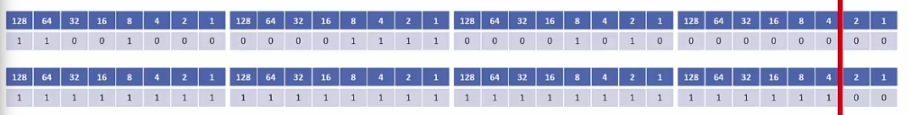
\includegraphics[width=\width\textwidth]{./figs/2022-10-19-23-12-35.png}
            %\caption{}
        \end{figure}
    
    \item /30 supports 2 hosts.
    \item 200.15.10.0 to 200.15.10.95 are already in use, so out network addresses will be 200.15.10.96.
    \item The network address goes up in values of 4, so the next one is 200.15.10.100.
    \item Our broadcast address is 200.15.10.99.
    \item Valid host addresses are 200.15.10.97 to 200.15.10.98.
\end{itemize}

\subsection{Network topology diagram}
\begin{itemize}
    \item Revisit the network diagram again:
        \begin{figure}[H]
            \centering
            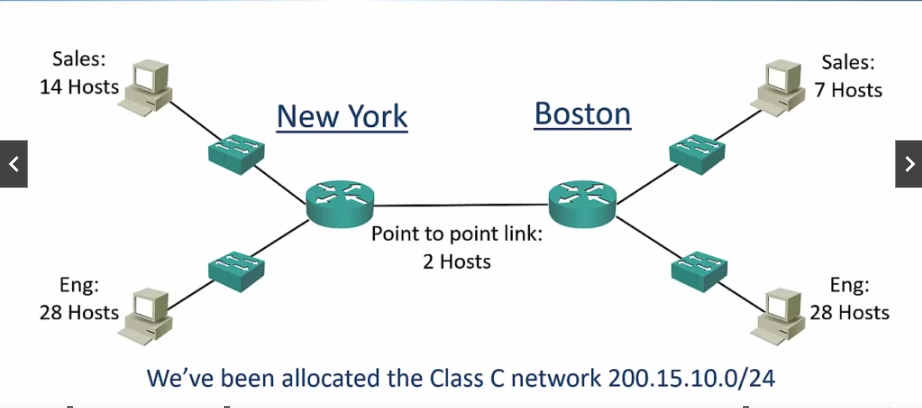
\includegraphics[width=\width\textwidth]{./figs/2022-10-19-23-21-23.png}
            %\caption{}
        \end{figure}
    
    \item Update the diagram with the IP address information for each subnet.
    \item Also enter the IP address on the router.
    \item The default gateway address should be the first available address in each subnet.
    \item It looks like this:
        \begin{figure}[H]
            \centering
            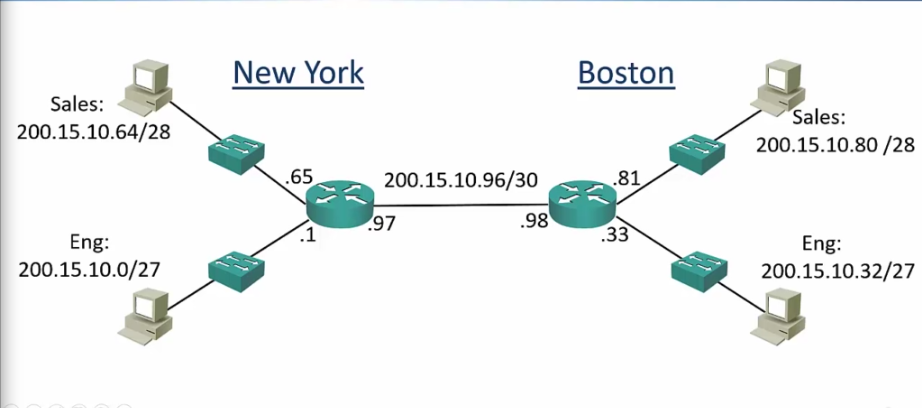
\includegraphics[width=\width\textwidth]{./figs/2022-10-19-23-21-58.png}
            %\caption{}
        \end{figure}
\end{itemize}

%%%%%%%%%%%%%%%%%%%%%%%%%%%%%%%%%%%%%%%%%%%%%%%%%%%%%%
\section{Subnetting Large Networks Part 1}
\begin{itemize}
    \item Given the class B 135.15.0.0/16
        \begin{figure}[H]
            \centering
            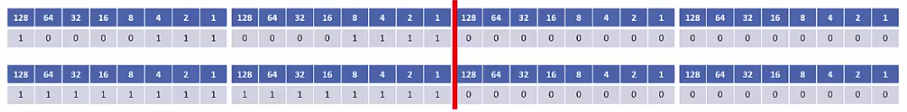
\includegraphics[width=\width\textwidth]{./figs/20230126151741.png}
            %\caption{}
        \end{figure}
    
    \item If we subnet this in /29 subnets, we have 3 bits for host addressing. This allows 6 hosts per network ($2^3-2$), the same as if we used /29 with a class C address.
    \item Because we were allocated a Class B /16 address range, we have 13 bits for network addresses. This allows for 8292 subnets ($2^{13}$)
\end{itemize}

\subsection{Examples}
\begin{itemize}
    \item Example 1: For the IP address 135.15.10.138/29, what is the network address, broadcast address, and range of valid IP addresses.
        \begin{figure}[H]
            \centering
            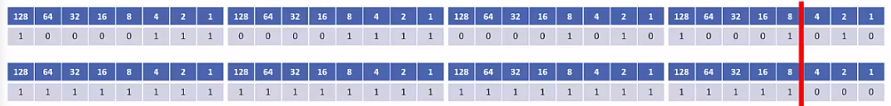
\includegraphics[width=\width\textwidth]{./figs/20230220135938.png}
            %\caption{}
        \end{figure}
        \begin{itemize}
            \item Notice in the above figure, the lower binary word is the subnetmast, since it has a contigous stream of 1's and then three zeros. The upper is the ip address.
            \item Thus the broadcast address is simply the ip in which the last 3 binary digits is 1, the network is when the last three digits are 0:
                \begin{itemize}
                    \item The base IP: 135.15.10.138 = 10000111.00001111.00001010.10001010
                    \item Network address: 10000111.00001111.00001010.10001000 = 135.15.10.136
                    \item Broadcast address: 10000111.00001111.00001010.10001111 = 135.15.10.143
                    \item Valid hosts: from the network address to the broadcast address - 2: 10000111.00001111.00001010.10001001 - 10000111.00001111.00001010.10001110 = 135.15.10.137 - 135.15.10.142
                \end{itemize}
        \end{itemize}
\end{itemize}

%%%%%%%%%%%%%%%%%%%%%%%%%%%%%%%%%%%%%%%%%%%%%%%%%%%%%%
\section{Subnetting Large Networks}
Example: class A on the third octet.
\begin{itemize}
    \item We are allocated a class A 60.0.0.0/8:
        \begin{figure}[H]
            \centering
            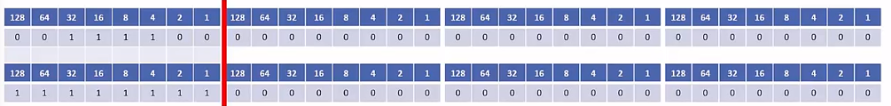
\includegraphics[width=\width\textwidth]{./figs/20230220165003.png}
            %\caption{}
        \end{figure}
        \begin{itemize}
            \item If we subnet this into fixed size subnet masks using /19, how many subnets do we have?
            \begin{itemize}
                \item The answer is /19 means we have 32-19 bits, or 13 bits for host addressing. This means we can reference up to $(2^{13}-2)$.
                \item This because we were allocated a class A /8 address range, we have 11 bits for network addresses, or $2^{11}=2048$ subnets.
                    \begin{figure}[H]
                        \centering
                        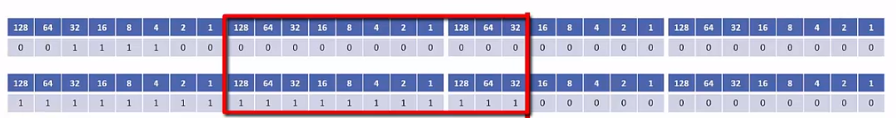
\includegraphics[width=\width\textwidth]{./figs/20230220184630.png}
                        %\caption{}
                    \end{figure}
            \end{itemize}
        \end{itemize}
    \item The IP address 60.15.10.75/19, what is the network address, broadcast address, adn range of valid IP addresses?
        \begin{figure}[H]
            \centering
            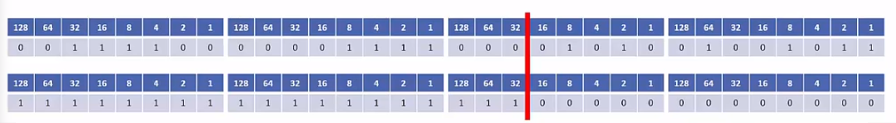
\includegraphics[width=\width\textwidth]{./figs/20230220184754.png}
            %\caption{}
        \end{figure}
        \begin{itemize}
            \item Notice that the line is after the 32, so the network address goes up in multiples of 32.
            \item Network address: 60.15.0.0
            \item Next network address: 60.15.32.0
            \item Broadcast address: 60.15.31.255
            \item Valid host addresses: 60.15.0.1 - 60.15.31.254.
        \end{itemize}
    
    \item You have been asked to subnet the 134.65.0.0 network into six different networks.
        \begin{figure}[H]
            \centering
            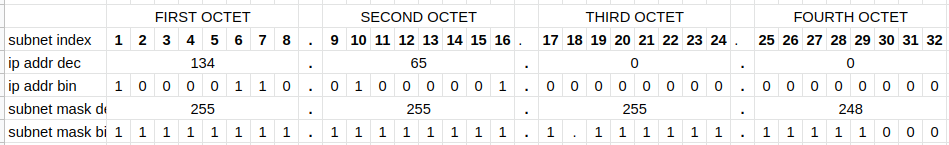
\includegraphics[width=\width\textwidth]{./figs/20230220190745.png}
            %\caption{}
        \end{figure}
        \begin{itemize}
            \item 134.65.0.0 is a class B network so we'll be subnetting on the third octet to get 6 subnets.
            \item 3 bits would provide 8 subnets $2^3$
            \item So the answer is /19 or 255.255.224. Since the subnet mask provided by class B ip addresses specify that the network address is the first 2 octets, we extend the subnet mask by three bits of the third octet the required 8 subnets.
            \item Network addresses would be 134.65.0.0, 134.65.32.0, 134.65.64.0, etc.
            \item 8190 hosts in each subnet $2^{13}-2$
        \end{itemize}
\end{itemize}

\subsection{Subnetting question categories}
\begin{itemize}
    \item Most exam questions will have the following format:
        \begin{itemize}
            \item Given a network requirement of 'x' amount of subnets and 'y' amount of hosts per subnet, what network addresses and subnet mask should be used for each subnet?
            \item Given a particular IP address and subnet mask, calculate: 
                \begin{itemize}
                    \item The subnet's network address. 
                    \item The broadcast address.
                    \item The range of valid host IP addresses.
                \end{itemize}
        \end{itemize}
\end{itemize}

%%%%%%%%%%%%%%%%%%%%%%%%%%%%%%%%%%%%%%%%%%%%%%%%%%%%%%
\section{Private IP addresses part 1}
\begin{itemize}
    \item Private addresses were documented by the IETF (Internet Engineering Task Force), when this organization documents anything it issues a RFC which stands for Request For Comment, basically its calling for peer reviewing of the documentation, so other engineers can comment and suggest improvements.
    \item The RFC 1918 specifies private IP address ranges which are not routable on the public internet.
        \begin{itemize}
            \item It is not common to memorize RFC numbers, but most engineers just know about RFC 1918 for private addresses, it is common terminology.
        \end{itemize}

    \item RFC 1918 Private Addresses:
        \begin{itemize}
            \item When the internet was thought out, there was some situations in which you wanted some IP addresses to not be connected to the internet. 
            \item For example in a company, you have a LAN that is not connected to the internet. 
            \item So private addresses were designed to have no connectivity to the internet.
            \item A publich IP, in contrast, costs money. So if you don't require IPs to connect to the internt it would be a waste of money and a potential vulnerability threat to use public. Instead use private.
            \item An example of organizations that use this are banks: it makes sense that banks would want to a part of their network to be completely cut off the internt for security reasons. They would use private IP addresses there. 
            \item There is a range of private addresses in each address class:
                \begin{itemize}
                    \item 10.0.0.0 - 10.255.255.255: class A /8 subnet mask.
                    \item 172.16.0.0 - 172.31.255.255: class B /12 subnet mask.
                    \item 192.168.0.0 - 192.168.255.255: class C /16 subnet mask.
                \end{itemize}
        \end{itemize}
    
    \item Example of when we would use private addresses:
        \begin{itemize}
            \item Given the following topology environment:
                \begin{figure}[H]
                    \centering
                    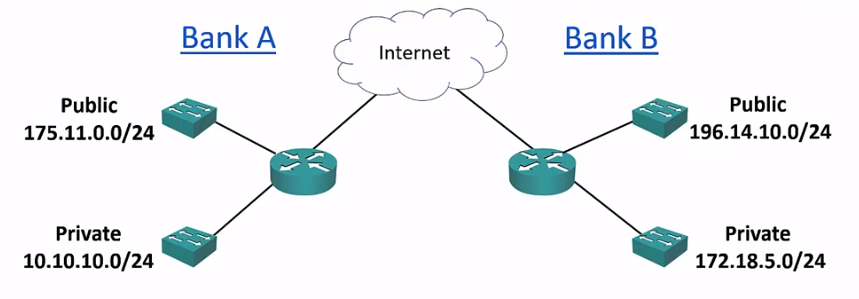
\includegraphics[width=\width\textwidth]{./figs/20230221142215.png}
                    %\caption{}
                \end{figure}
            
            \item Bank A has a public and a private part of their network. The public one is used to access the internet (175.11.0.0/24). The private LAN cannot access the internet (10.10.10.0/24). 
            \item The same configuration is followed by Bank B. Notice that the public LAN of each bank is different, and that is to be expected, but the private is exactly the same. This is not a problem since these IPs are only significant in each bank's network. So no conflict here. They can't use the same public addresses since they would conflict.
        \end{itemize}
    
    \item The IPv4 Global Address Space Problem, the solution IPv6:
        \begin{itemize}
            \item Let's revisit the problem of the IPv4 design.
            \item Remember that the class A loopback address 127.0.0.0 removed millions of ips that could been allocated to organizations? The designers of the ipv4 protocol did not forsee that the IPs would soon run out and the available 4.3 billion addresses would not be enough.
            \item They ran out of addresses. The internet authorities started to predict address exhaustion in the late 1980's, and IPv6 was developed in the 90's as the long term solution.
            \item IPv6 uses a 128 bit (16 byte) address, compared to IPv4's 32 bit (4 byte) address.
            \item IPv6 provides more than $7.9\times 10^{28}$ times as many addresses as IPv4. Keep in mind that because 16 bytes and 4 bytes there is an exponential difference, its not just "4 times as large", its actually exponentially bigger ($7.9\times 10^{28}$ bigger to be exact).
        \end{itemize}
    
    \item The IPv6 problem and NAT:
        \begin{itemize}
            \item There is not a seamless migration path from the IPv4 and IPv6.
            \item Changing from ipv4 to ipv6 is not easy, one is not compatible with the other, so until organizations can upgrade from ipv4 to ipv6, a technology (a work around) was developed as a temporary solution to this, its called NAT.
            \item NAT stands for Network Address Translation, and it basically works like this:
                \begin{itemize}
                    \item Let's say that we have an organization that has the private IP addresses mentioned in the last example. So it has a public and a private LAN. With NAT the private addresses can communicate with the internet as if they were public. So the organization can use the RFC 1918 private IP addresses which are not publicly routable, so they don't work in the public internet. On the way out, NAT converts the communications coming from the private IPs to public IP addresses. 
                    \item So when then the internet trafic goes out from your private IP address, NAT transforms it to a public IP and the internet can send trafic back through NAT.
                    \item Many hosts on the inside that are using the RFC 1918 private IP addresses can share a single public IP on the outside.
                \end{itemize}    
        \end{itemize}
    
    \item Now for an example of private IP addresses and NAT:
        \begin{itemize}
            \item Given the following topology: 
                \begin{figure}[H]
                    \centering
                    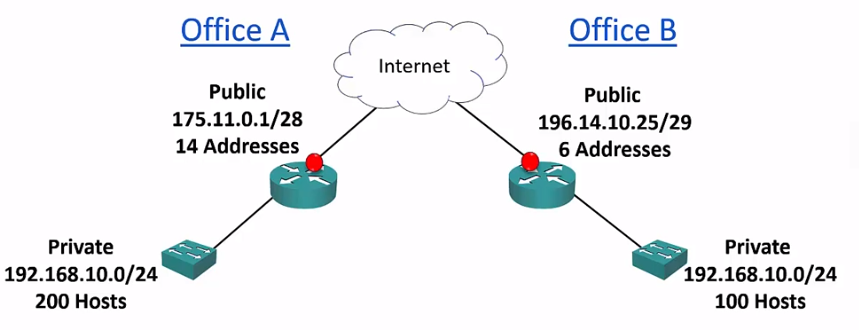
\includegraphics[width=\width\textwidth]{./figs/20230221143926.png}
                    %\caption{}
                \end{figure}
            
            \item Office A and B have the same configuration, a range of public and private IP addresses. The private IPs cannot communicate with the internet. Not yet...
            \item So NAT will translate the private IPs whenever they are communicating with anybody on the internet. This saves lots of addresses in the ipv4 public address space. And it saves organization's money because public IPs cost money, we can have just one, and have loads of private IPs, and just communicate through that one public IP using NAT.
        \end{itemize}
\end{itemize}

%%%%%%%%%%%%%%%%%%%%%%%%%%%%%%%%%%%%%%%%%%%%%%%%%%%%%%
\section{Private IP addresses part 2}
\begin{itemize}
    \item Today's networks:
        \begin{itemize}
            \item Back in the 2000s everybody was saying that they were living the final days of ipv4. But the truth is that it has not happened, almost everybody is using ipv4 with NAT using RFC 1918 private addresses. 
            \item There are several reasons for this, first there is security benefit of hiding hosts inside a private LAN, the hosts do not have a privately routable IP address. Another reason is that ipv6 has not completely taken over is because most people have more experience using ipv4. Ipv6 is actually a very different format, so most people are not familiar to the format of ipv4.
            \item Despite this, ipv6 is still found in some companies, primarily service provider networks, mobile services and large countries that adopted the internet later such as India and China.
            \item Spare public IPv4 addresses were exhausted in 2011 so IPv6 is still the future path. It will be a slow process of adoption but eventually ipv4 will be deprecated and ipv6 will completely take hold.
            \item Subnetting is used in RFC 1918 private IP addressing to optimise performance and security.
            \item You also need to understand subnetting to be able to troubleshoot IP.
            \item Because most people use the private IP RFC 1918, it is common to see /24 subnets being used for end hosts, /30 subnetting for point to point links, and /32 for loopback. Remember that if we use the private IPs with NAT, we can have all the range of IPs as if they were ours, so all the possible values from 0.0.0.0 to 255.255.255.255 is ours to do with as we please. We communicate trafic with the internet using our public IP RFC 1918.
            \item Using many subnets in the same networks is called VLSM is more common in enterprises which use public IP addresses on their side of networks and need to maximize their use.
        \end{itemize}
    
    \item Contiguos addresses and route summarization:
        \begin{itemize}
            \item Even if you are using private IPs, route summarisation still needs to be used.
            \item The folllowing example:
                \begin{figure}[H]
                    \centering
                    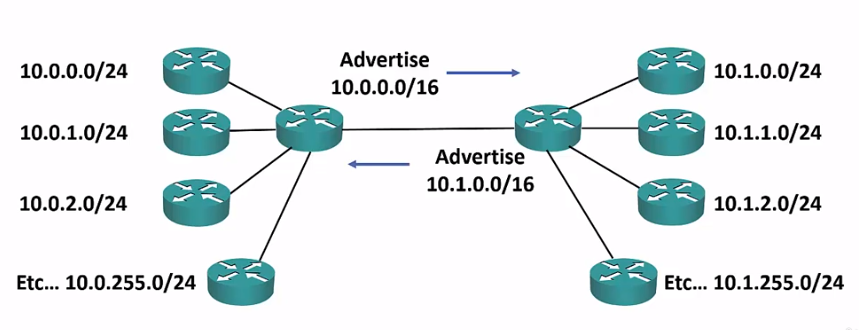
\includegraphics[width=\width\textwidth]{./figs/20230221223230.png}
                    %\caption{}
                \end{figure}
            
            \item Notice that the advertise address in the center left router is 10.0.0.0/1y6, this is because it is the common bits that all the IPs have, all of the IPs start with 10.0. Same on the right side, all IPs start with 10.1. 
            \item So when using private IPs you must be careful allocating them, always look to allocate them in contigous blocks. It would be a mistake to not allocate them in contigous blocks like this:
                \begin{figure}[H]
                    \centering
                    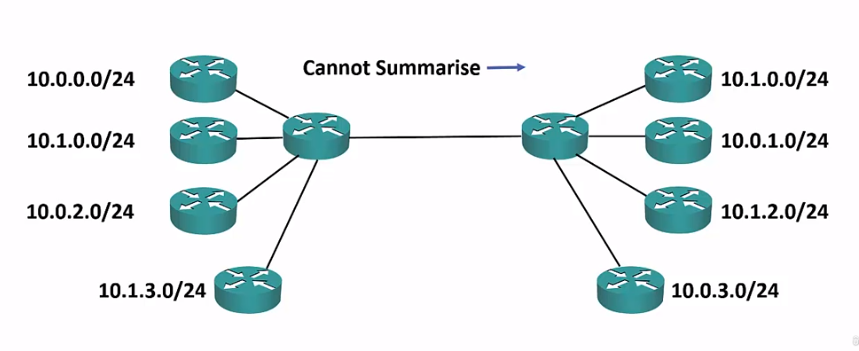
\includegraphics[width=\width\textwidth]{./figs/20230221223458.png}
                    %\caption{}
                \end{figure}
            
            \item Notice in the above image that we cannot summarize because the IPs don't have much in common, in this scenario the routers would have to have a list of all routers complete addresses. The IPs dont start with 10.0, but are different i.e. 10.1, 10.0. so you cannot summarise them. Always plan your private IP addressing address space.
        \end{itemize}
\end{itemize}

%%%%%%%%%%%%%%%%%%%%%%%%%%%%%%%%%%%%%%%%%%%%%%%%%%%%%%
\section{Where to get more subnetting practice?}
\begin{itemize}
    \item Consider using this to study for CCNA.
    \item \url{http://www.subnettingquestions.com/}
        \begin{itemize}
            \item For questions on subnetting.
            \item Every refreshing of the site will give you a new question.
        \end{itemize}
    \item \url{http://www.subnetting.org/}
    \item \url{https://subnettingpractice.com/}
    \item Search in google for Subnetting calculators and questions.
\end{itemize}